\section*{Trust}

\subsection*{Answering Road Map}


\usetikzlibrary{shapes.geometric, arrows.meta, positioning}

\tikzstyle{startstop} = [rectangle, rounded corners, minimum width=2cm, minimum height=1cm,text centered, draw=black, fill=blue!20]
\tikzstyle{process} = [rectangle, minimum width=2cm, minimum height=1cm, text centered, draw=black, fill=orange!30]
\tikzstyle{decision} = [diamond, aspect=2, minimum width=3.5cm, minimum height=1.2cm, text centered, draw=black, fill=green!30]
\tikzstyle{arrow} = [thick,->,>=stealth]

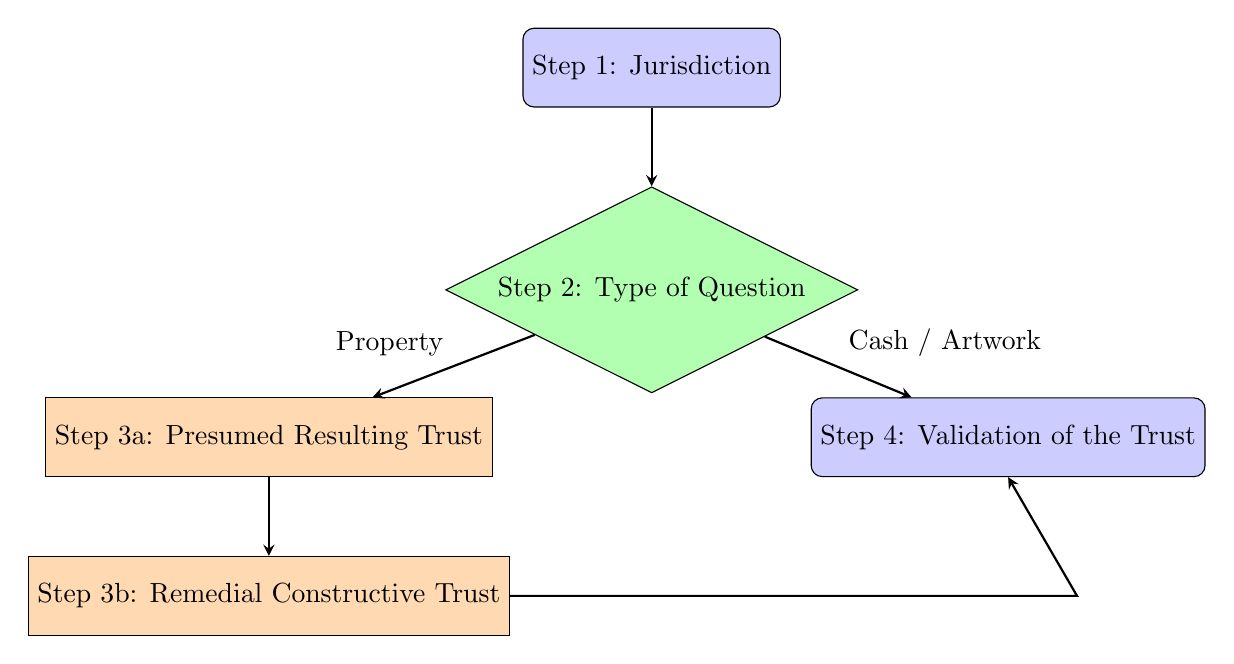
\begin{tikzpicture}[node distance=1cm and 1.5cm]

% Nodes
\node (start) [startstop] {Step 1: Jurisdiction};
\node (step2) [decision, below=of start] {Step 2: Type of Question};
\node (step3a) [process, below left =1 cm of step2] {Step 3a: Presumed Resulting Trust};
\node (step3b) [process, below=of step3a] {Step 3b: Remedial Constructive Trust};
\node (step4) [startstop, below right =1cm of step2] {Step 4: Validation of the Trust};

% Arrows
\draw [arrow] (start) -- (step2);
\draw [arrow] (step2) -- node[anchor=south east] {Property} (step3a);
\draw [arrow] (step3a) --  (step3b);
\draw [arrow] (step2) -- node[anchor=south west] {Cash / Artwork} (step4);
%\draw [arrow] (step3b) -- (step4);
\draw [arrow] (step3b.east) --++(7.20,0)-- (step4.south);

% Optional connection (e.g., an alternate path or comparative analysis)
%\draw [arrow, dashed] (step2) -- (step3b);
%\draw [arrow, dashed] (step3b) |- (step4); % uncomment if 3b leads to 4

\end{tikzpicture}



\section*{Jurisdiction}
The jurisdiction is QLD. Therefore, in Trust, when talking about formality, Only land and will need to satisfy the law requirement. otherwise as long as satisfy the equity requirement is good enough. the trust formality need to follow:
\begin{itemize}
    \item inter vivos
        \begin{itemize}
            \item Property Law Act 1974 (Qld) s 11
            \item Secretary of the Department of Social Security v James
        \end{itemize}
    \item testamentary trusts
        \begin{itemize}
            \item Succession Act 1981 (Qld) s10
            \item Property Law Act 1974 (Qld) s11
        \end{itemize}
    \item Equity
        \begin{itemize}
            \item Milroy v Lord
            \item Property Law Act 1974 )Qld) s 200(1)
        \end{itemize}
\end{itemize}

\section*{Presumed Resulting Trust}
\begin{enumerate}
    \item look at the intentions at the time of purchases
    \item look at relationship
    \item what about non-financial contributions
    \item if no relationship no contributions. are party holding an constructive trust for other. 
    \begin{description}
        \item[Note:]when answering this type questions, starts with Calverly v Green, then Muschinski v Dodds, then Baumgartner v Baumgartner
    \end{description}
\end{enumerate}


\section*{Constructive Trust}
\begin{enumerate}
    \item Element of unconscionability
        \begin{description}
            \item[Deane J in Muschinski v Dodds]Equity requires that the rights and obligations of the parties be adjusted to compensate for the disproportion between their contributions”
        \end{description}
    \item Applying Muschinski v Dodds and Baumgartner v Baumgartner (take into account all contributions);
\end{enumerate}

\section*{Validation of the Trust}
An express trust can be created in one of two ways:
\begin{enumerate}
    \item Declaration of trust where settlor declares himself to hold property on trust for a beneficiary
    \item transfer of property $+$ intention for transferee to be beneficial owners.
\end{enumerate}
Necessary elements of a trust include:
\begin{itemize}
    \item Certainty of intention
    \item certainty of subject matter
    \item Certainty of objects
    \item Formalities
\end{itemize}

\subsection*{Intention}
Express trust is only upheld if there is certainty of intention to create trust on the part of the holder.
\begin{enumerate}
    \item If language is clear then determine the intention from the language
    \item If the language is ambiguous, look to:
    \item Whole of trust instrument and define the ambiguous language in light of that 
        \begin{description}
            \item[Dean v Cole:]No precatory words 
            \item[Hayes:]Context shows intended obligation
        \end{description}
    \item Look to the nature of transaction and relationships 
        \begin{description}
            \item[Bahr v Nicolay] Equitable, unconscionability-based
            \item [Trident per Deane J]Real expectations and fairness require recognition of obligation
        \end{description}

\end{enumerate}

\subsubsection*{Common Precatory Words in Trust Law}
Precatory words are expressions of wish, hope, or desire used in wills or trust documents that do not create a binding trust obligation unless a clear intention to create a trust can be found.

\vspace{0.5cm}

\begin{tabular}{@{}ll@{}}
\hline
\textbf{Precatory Word or Phrase} & \textbf{Interpretation in Trust Law} \\
\hline
``I hope''                    & Expression of desire; not legally binding \\
``I wish''                   & Suggests moral expectation, not legal duty \\
``I desire''                 & Indicates intention, but not enforceable as a trust \\
``I request''                & Seen as a non-binding recommendation \\
``It is my intention that''  & May indicate purpose, but lacks obligation \\
{}& unless context supports a trust \\
``In the belief that''       & Assumes outcome; does not impose obligation \\
``I would like''             & Non-binding expression of preference \\
``I am confident that''      & Reflects hope, not duty \\
``To be at liberty to''      & Gives discretion, not a fiduciary obligation \\
``I recommend that''         & Merely advisory; insufficient to impose trust \\
\hline
\end{tabular}

\subsection*{Subject Matter}
Trustees must be able to clearly identify the property of the trust. In terms of its nature, any type of property—whether tangible or intangible—may form the subject matter of a trust, with the exception of future interests and mere expectancies. Regarding the quantum of the property, in the case of a fixed trust (as opposed to a discretionary trust), the specific entitlement of each beneficiary must be certain. If the trust property cannot be properly identified or is uncertain, the trust will be considered void.

\subsubsection*{Case Application}
\begin{itemize}
    \item Re Golay
        \begin{description}
            \item[Note:]can court use common sense to work it out the number. 
        \end{description}
    \item Hunter v Moss
        \begin{description}
            \item[Note:]Very clear number is good 
        \end{description}
    \item Re Goldcorp
        \begin{description}
            \item[Note:] need to segregate property from other property for there to be certainty of subject matter. For example: artwork.
        \end{description}
    \item White v Shortall
        \begin{description}
            \item[Note:] instead of needing to have homogenous property in separate trusts, could have it in one big trust that can be “certainly” identified and parties have an interest equal to part of it
        \end{description}
\end{itemize}

\subsection*{Object}
Beneficiary principle: trust must be enforceable by some person and controllable by court that means human needs to have a name, or a named pet, etc. If the trust is for a charitable purpose, we need to have two stage analogy approach.

\subsubsection*{Determine beneficiaries}
\begin{itemize}
    \item Fixed trust
        \begin{description}
            \item[Definition:]Trust where the rights of all beneficiaries are fixed by the trust deed
            \item[Application:]List of possible objects has to be  compiled or capable of compilation (“list certainty”)
            \item[West v Weston:]list certainty
        \end{description}
    \item Discretionary trust
        \begin{description}
            \item[Definition:]Trust where Trustees have a discretion to decide who among a
class of beneficiaries will receive a benefit and may also be able to decide the amount of the benefit to be paid
            \item[Application:]Trustee need only be able to determine with certainty whether any claimant is within the class (“in”/“out” test)
            \item[Re Barlow:]cannot determine family and friends
            \item[McPhail v Doulton and Re Gulbenkian’s Settlement] determine
        \end{description}
\end{itemize}

\subsubsection*{Determine trust purpose}
\begin{itemize}
    \item Non-Charitable purpose
        \begin{itemize}
            \item beneficiary principle -- express trusts must be for a person/persons(Morice v Bishop of Durham)
            \item Tombs and animals ( Pedulla v Nasti)
            \item Gifts to unincorporated associations. 
        \end{itemize}
    \item Charitable purposes
        \begin{itemize}
            \item Two stage test
                \begin{description}
                    \item[Stage one:] Lord Macnaghten in Pemsel 
                        \begin{itemize}
                            \item relief of poverty
                            \item advancement of education
                            \item advancement of religion
                            \item beneficial to the community
                        \end{itemize}
                    \item[Stage Two:]Is it one of the purposes in the Statue of Charitable Uses 1601 (Imp) Preamble?
                        \begin{itemize}
                            \item Trusts Act 1973 (Qld) s 103(1)
                            \item Incorporated Council of Law Reporting (Qld) v Federal Commissioner of Taxation (1971) 125 CLR 659 at 666-667 (Barwick CJ) – “it is a matter of judgment ... ‘within the spirit and intendment’”
                            \item Charities Act 2013 (Cth) section 12
                        \end{itemize}
                \end{description}
        \end{itemize}
\end{itemize}

\subsection*{Formality}
\begin{itemize}
    \item At Law
        \begin{itemize}
            \item  No land - no writing required - Property Law Act s11(1)
            \item It is a will – must satisfy the writing requirements in the
Succession Act s 10
        \end{itemize}
    \item In Equity “everything necessary”
        \begin{itemize}
            \item Milroy v Lord
            \item Property Law Act 1974 (Qld) s 200(1)
        \end{itemize}
\end{itemize}

\subsubsection*{Failed Bequest}
If any of the validation elements failed, go back to the successor entitle or automatic resulting trust. 

\subsection*{Breach of Trust}
A “breach of trust” is: A trustee acting, or omitting to act, in contravention of their trust duties
\begin{itemize}
    \item According to the trust deed
    \item According to the duties attached to the office of trustee
        \begin{description}
            \item[examples]
                \begin{itemize}
                    \item General duties
                    \item Duty to account and provide information
                    \item Duty to administer the trust personally
                    \item Duty to avoid a conflict of interest
                    \item Duty to act impartially
                    \item Duty to invest trust property
                    \item Duty to pay correct beneficiaries
                \end{itemize}
        \end{description}
    \item Acting in bad faith or for ulterior purposes

    \item A trustee acting in excess of their powers, or omitting to exercise their powers(Hourigan v Trustees Executors and Agency Co Ltd )
        \begin{itemize}
            \item Trust Power
            \item Mere Power
        \end{itemize}
\end{itemize}

\subsubsection*{Defense}
\begin{itemize}
    \item Specific provisions in the trust instrument limiting the liability
    \item Disclosure and informed consent
        \item Delay in bringing an action
    \item  Court also has power to relieve trustees from personal liability (Trusts Act 1973 (Qld) s 76)

\end{itemize}

\subsubsection*{Remedy}
\begin{itemize}
    \item Equitable compensation
    \item Interest
    \item Account of profits
    \item Injunction
    \item Constructive trust
    \item Tracing in specie
    \item Tracing to mixed or converted funds
    \item The in personam remedy in Re Diplock and the Trusts Act 1973 (Qld) s 113
\end{itemize}




